%\usepackage{tikz}
\begin{figure}[h]
\centering
\caption{Diagram for a three-layered network}\vspace*{2mm}\label{fig:diagram}
\begin{boxedminipage}{9.2cm}
\def\layersep{3.5cm}
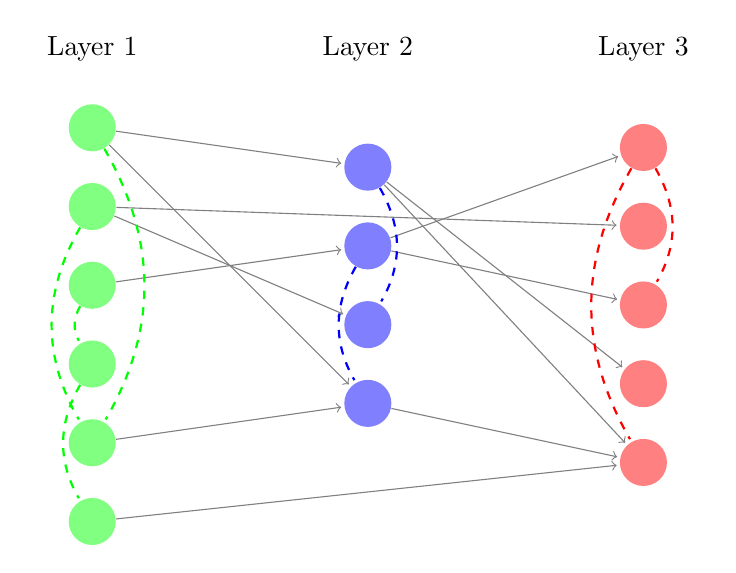
\begin{tikzpicture}[shorten >=1pt,->,draw=black!50, node distance=\layersep]
    \tikzstyle{every pin edge}=[<-,shorten <=1pt]
    \tikzstyle{neuron}=[circle,fill=black!25,minimum size=17pt,inner sep=0pt]
    \tikzstyle{input neuron}=[neuron, fill=green!50];
    \tikzstyle{output neuron}=[neuron, fill=red!50];
    \tikzstyle{hidden neuron}=[neuron, fill=blue!50];
    \tikzstyle{annot} = [text width=4em, text centered]

    % Draw the input layer nodes
    \foreach \name / \y in {1,...,6}
    % This is the same as writing \foreach \name / \y in {1/1,2/2,3/3,4/4}
        \node[input neuron] (I-\name) at (0,-\y) {};

    % Draw the hidden layer nodes
    \foreach \name / \y in {1,...,4}
        \path[yshift=-0.5cm]
            node[hidden neuron] (H-\name) at (\layersep,-\y cm) {};

    % Draw the output layer node
    \foreach \name / \y in {1,...,5} 
	   \path[yshift=-0.25cm]
		   node[output neuron] (O-\name) at (2*\layersep, -\y cm) {};
	    
    % % connect node in Layer 1 and Layer 2
    \path (I-1) edge (H-1); \path (I-1) edge (H-4);
    \path (I-2) edge (H-3);
    \path (I-5) edge (H-4);
    \path (I-3) edge (H-2);
    

    % Connect node in Layer 2 and Layer 3
    \path (H-2) edge (O-1); \path (H-2) edge (O-3);
    \path (H-1) edge (O-4); \path (H-1) edge (O-5);
    \path (H-4) edge (O-5);
    
    %  connect node in Layer 1 and Layer 3
    \path (I-2) edge (O-2); \path (I-6) edge (O-5);
    
    %  add within-layer connections
    \path[-,dashed, green,thick,bend left] (I-1) edge (I-5);
    \path[-,dashed, green,thick,bend right](I-2) edge (I-5);
	\path[-,dashed, green,thick,bend right](I-3) edge (I-4);
    \path[-,dashed, green,thick,bend right](I-4) edge (I-6);
    
    \path[-,dashed, blue,thick,bend left] (H-1) edge (H-3);
    \path[-,dashed, blue,thick,bend right] (H-2) edge (H-4);
     
    \path[-,dashed, red,thick,bend left] (O-1) edge (O-3);
    \path[-,dashed, red,thick,bend right] (O-1) edge (O-5);
    
    % Annotate the layers
    \node[annot,above of=H-1, node distance=1.5cm] (hl) {Layer 2};
    \node[annot,left of=hl] {Layer 1};
    \node[annot,right of=hl] {Layer 3};
\end{tikzpicture}
\end{boxedminipage}
\end{figure}